\RequirePackage{docswitch}
% \flag is set by the user, through the makefile:
%    make note
%    make apj
% etc.
\setjournal{\flag}

\documentclass[\docopts]{\docclass}

% You could also define the document class directly
%\documentclass[]{emulateapj}

% Custom commands from LSST DESC, see texmf/styles/lsstdesc_macros.sty
\usepackage{lsstdesc_macros}

\usepackage{graphicx}
\graphicspath{{./}{./figures/}}
\bibliographystyle{apj}

% Add your own macros here:


\author{Rick Kessler,  Rahul Biswas, Alex Boucard, Mi Dai, Renee Hlozek,
Saurabh W.~Jha, Lluis Galbany, Emille Ishida, Ashish Mahabal, Kaisey Mandel, Rafael Martinez-Galarza, Daniel Mutukrishna, Tina Peters, Kara Ponder}

% ======================================================================

\begin{document}

\title{The Photometric LSST Astronomical Time-series Classification Challenge (PLAsTiCC): Data set}

%\maketitlepre

\begin{abstract}
The Photometric LSST Astronomical Time Series Classification Challenge (PLAsTiCC) is an open data challenge to classify simulated astronomical time series data in preparation for the data from the Large Synoptic Survey Telescope (LSST), that will achieve first light in 2022. We briefly describe the PLAsTiCC data set that will be tested by the Kaggle team. This note will be updated for the full release of the data to the community.

\end{abstract}

% Keywords are ignored in the LSST DESC Note style:
\dockeys{}

\maketitlepost

% ----------------------------------------------------------------------
% 

\section{Introduction}
\label{sec:intro}
PLAsTiCC is a large data challenge where participants are asked to \textit{classify astronomical time series data}. These simulated time series data, or `light curves' are measurements of flux in different astronomical wavelength bands as a function of time, and are simulations of what we expect from the upcoming LSST survey. For each object, the data provided includes summary information: its position on the sky, an estimate of its observed redshift (which correlates with its distance away from Earth), and other properties of the sky near the object. In addition, the light curve \textit{photometry} data on the object is a table of fluxes at different times of observation, and at different wavebands (i.e. the average energy of the light within a range of wavelengths). We go into more detail in the following section about the astronomical terminology used here.

In Figure~\ref{fig:lc}, we show three light curves for different types of objects.

\begin{figure*}[htbp!]
\begin{center} 
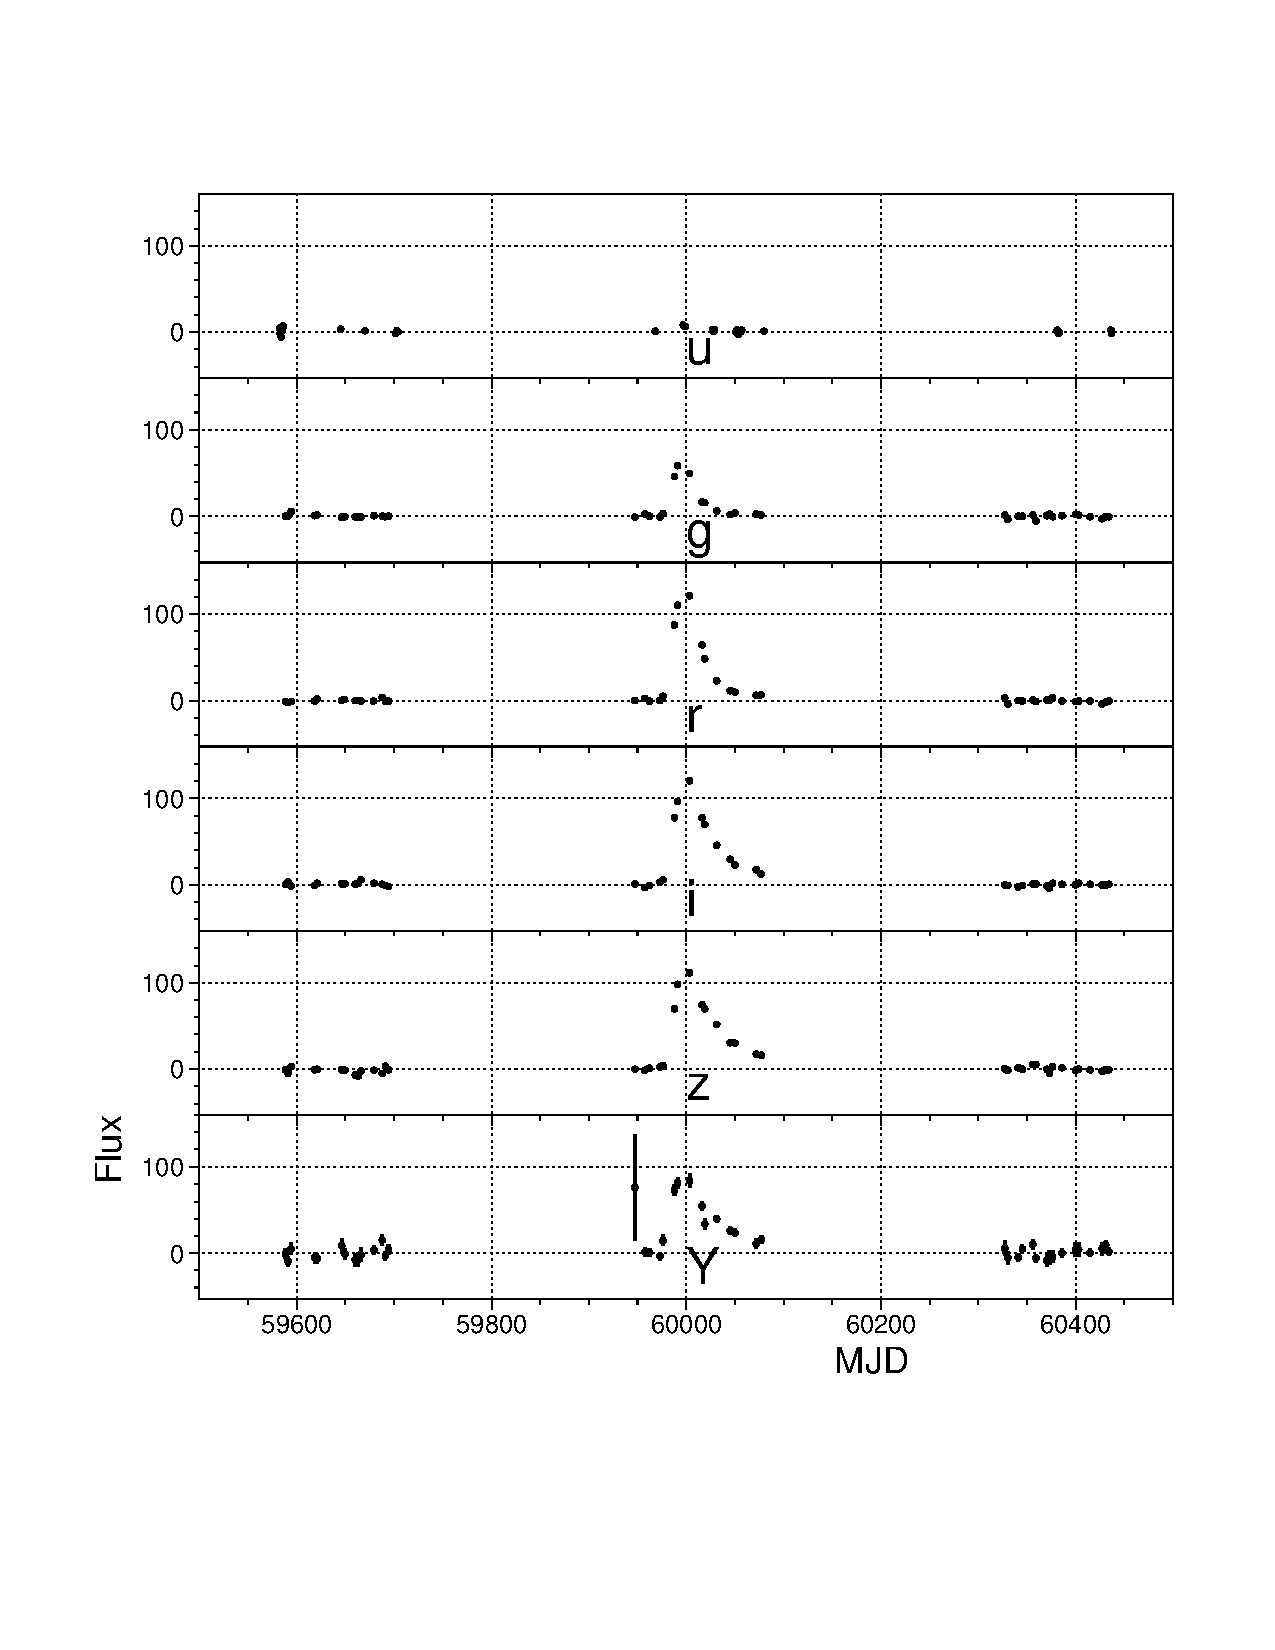
\includegraphics[scale=0.4, trim = 15mm 45mm 10mm 20mm, clip]{figures/lcplot_model01a.pdf}
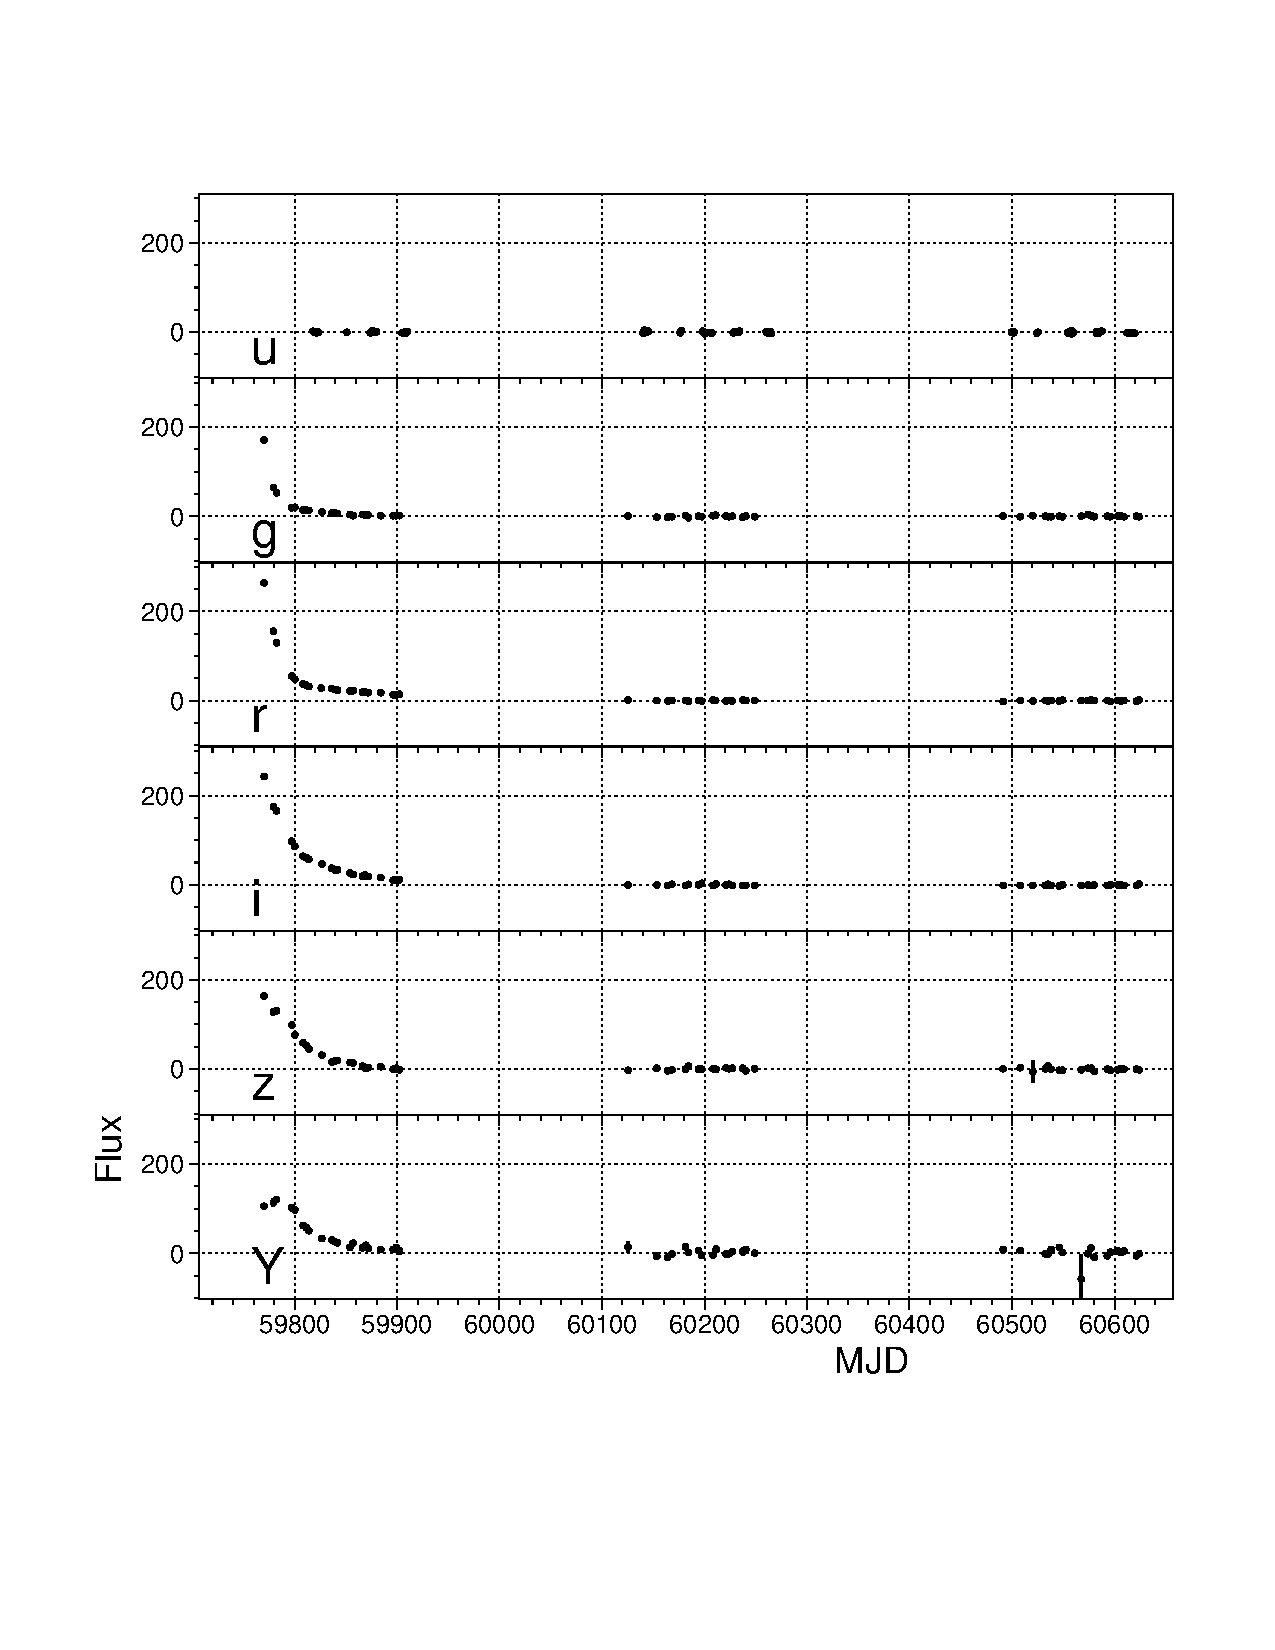
\includegraphics[scale=0.4,trim = 15mm 45mm 10mm 20mm, clip]{figures/lcplot_model01b.pdf}
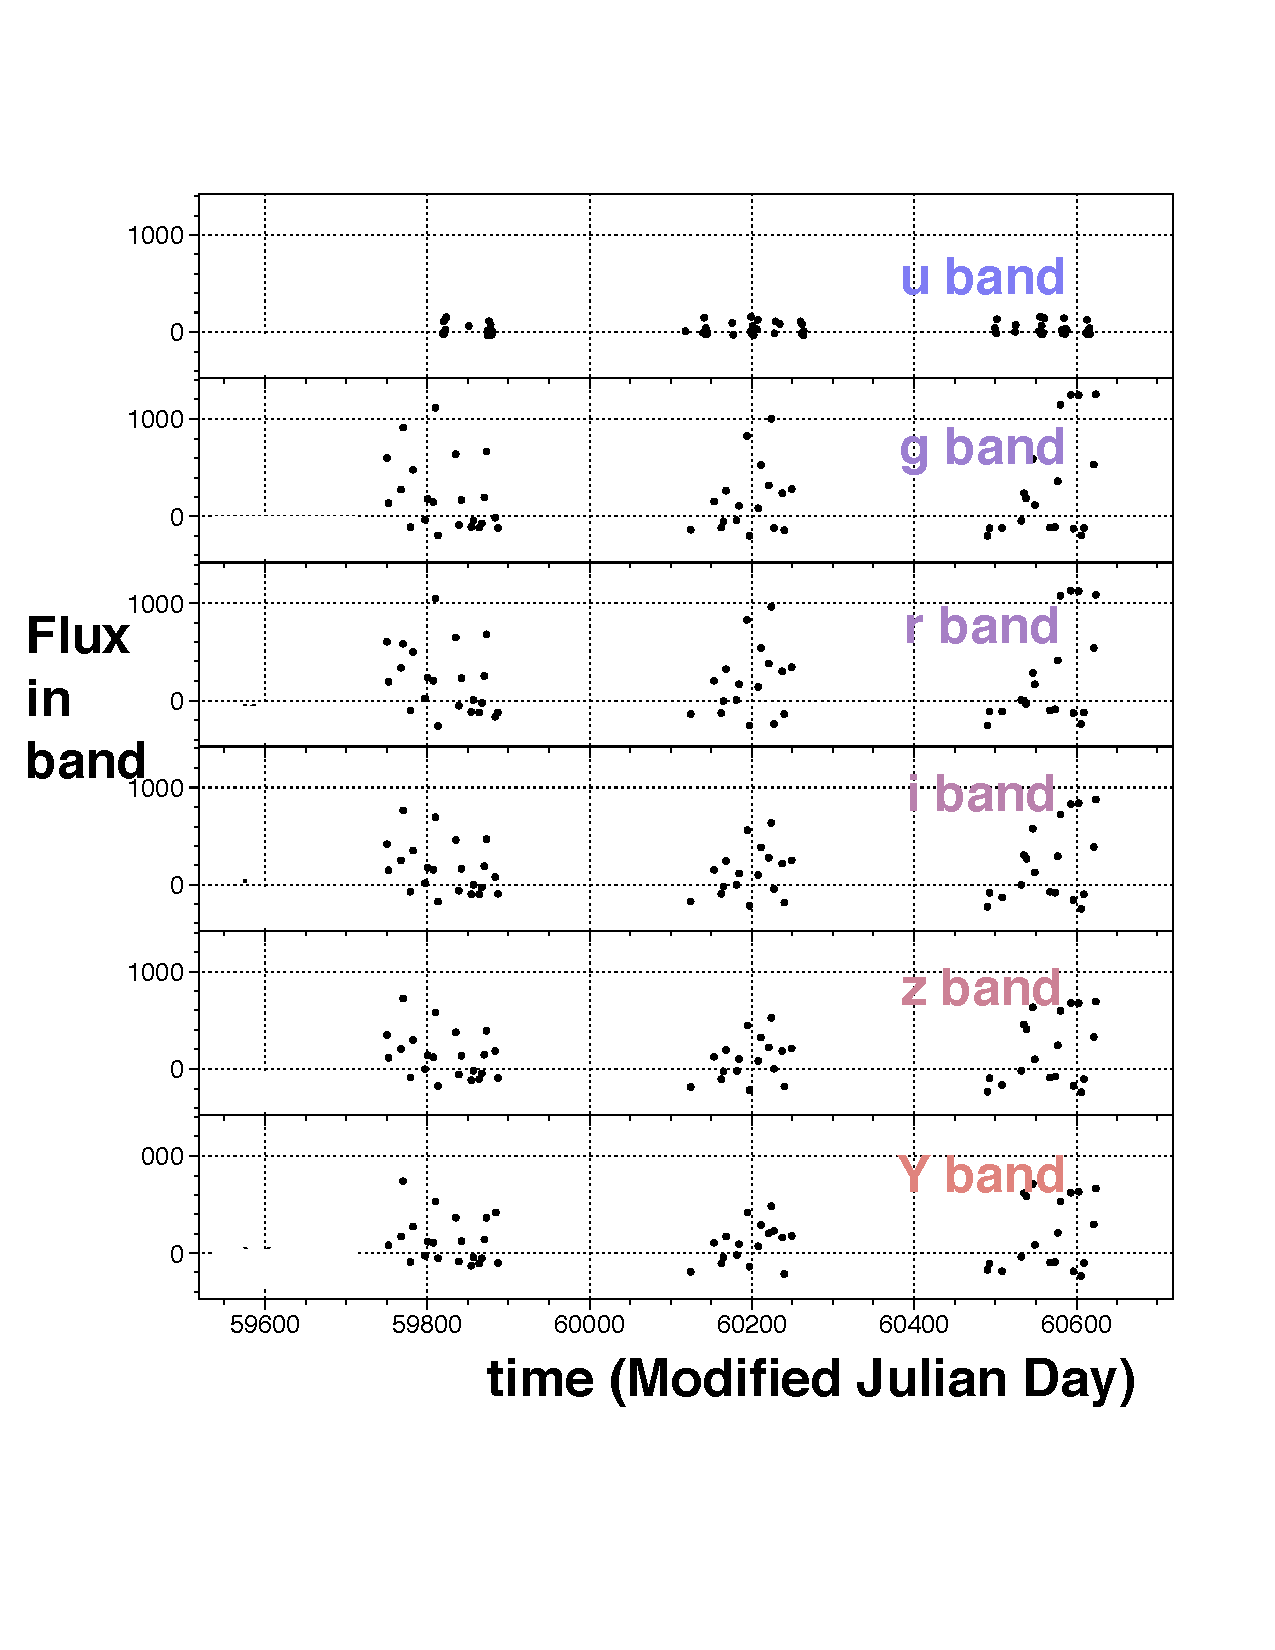
\includegraphics[scale=0.4,trim = 15mm 45mm 10mm 20mm, clip]{figures/lcplot_model80.pdf}
\caption{Example light curves in the PLAsTiCC data set. The three example objects display different changes in flux with time typical of real-world objects. They are either transient, and brighten suddenly before fading again into obscurity (top row) or they display flux variability, brightening and fading (bottom figure). This brightening can either be periodic or aperiodic. The top row also illustrates that the brightening of the flux can occur near the edges of the survey, and therefore may not include the full time period of brightening for the object. In addition, all three panels show that seasonal gaps and the instrument cadence of observations can introduce gaps in the light curve.\label{fig:lc}}
\end{center}
\end{figure*}
The users are asked to classify the data into XX classes, XX-1 of which are represented in the training sample. The final class designation of `other' is meant to capture objects that are hypothesized to exist but have never been observed and are thus not in the training set.


\section{Astronomy Background}
While we think of the night sky as static, it is filled with sources of light that vary in brightness on timescales from seconds and minutes to months and years. 

Some of these events are classified as \textit{transients}, and are the
observational consequences of a large variety of astronomical phenomena. For example, the cataclysmic event that occurs when a supernova explodes generates a bright signal that fades with time, but does not repeat.

Other events are classified as \textit{variables}, since they can vary their brightness in a periodic (or aperiodic) fashion, and originate from physical process governing high density regions of the Universe such as emission from the active galactic nuclei (AGN) at the hearts of galaxies, or as a result of geometric effects (e.g. eclipsing binary stars that alternately block out each others light from view).


These transient objects can provide important clues about themselves and their environment - as well as the evolution of the universe as a whole (e.g. type Ia supernovae provided the first evidence of the current accelerated expansion of the Universe which might be caused by dark energy). 

Each different type of transient and variable provides a different clue that helps us study how stars evolve, the physics of stellar explosions, the chemical enrichment of the cosmos, and the accelerating expansion of the universe.  Therefore, the proper classification of transients is a crucial task in observational astronomy - specially in the light of large data volumes expected for the next generation of astronomical surveys.

The main aim of this challenge is: \textit{can one classify astronomical transients and variables from a photometric light curve data set designed to mimic the data from the upcoming Large Synoptic Survey Telescope (LSST)?} Crucially, the classification will occur on a large test set, but the training data will be a small, and poorly representative training set, to mimic the challenges we face observationally.

\subsection{Different ways of observing astronomical objects}
Next we give more detail on LSST, and the challenge at hand. The two modes for characterising the light from the objects are called spectroscopy and photometry.
Spectroscopy measures the flux per wavelength interval and is the modern equivalent of using a prism to separate a beam of light in its composite (e.g. rainbow) colours. It is a high resolution measurement which allows us to identify emission/absorption features indicative of specific chemical elements present in the object.  Spectroscopy is also the primary tool that enables classification of astronomical transients and variables. Despite being paramount for the classification task, spectroscopy is an extremely time consuming process - with integration times ranging from 20 minutes to a few hours depending on the telescope and brightness of the source.

Given the volume of data expected from the upcoming large scale sky surveys, obtaining spectroscopy for every object is not sustainable. An alternative approach is to take an image of the object through different wavelength (band) filters, to determine the flux of the object. Classification is then performed on the light curves that result from those images.

Photometry records how bright the source is at a given moment. The photometric information is encoded as the flux (energy from the object). The photometric light curve has six pieces of information, namely the flux in six wavelength bands (named $ugrizY$) at any moment in time.
%, or the magnitude $m$ (the base-10 logarithm of the flux from the object):

%\begin{equation}
%F = 10^{-0.4m+11} + \mbox{noise}
%\end{equation}
These photometric wavelength band fluxes are the integrals of the spectrum over the filter bandpasses of atmosphere and of the instrument divided by the energy of photons in the central wavelength of the filter. A sequence of photometric observations made at different times is called a light curve. It measures how the energy of the source evolves with time and can also be used to characterize different types of astronomical transients. As a consequence, for each object we will have a number of light curves in each filter (or band). Wavelengths are measured in units of Angstrom ($\AA$), where $1\AA = 10^{-10} m.$ Each band corresponds to a `color', with a width of around 1000 $\AA$, with the full set ranging from $3000\AA$ (blue light) to $9000\AA$ (near infrared light).

The observations are affected by wavelength-dependent sky noise (due to e.g., moonlight and other sources). 
High-resolution spectroscopy carries thousands of information bits, and hence the challenge is to use the highly compressed photometric information to perform classification.

Unlike spectroscopy, photometry measures light from a large wavelength range simultaneously, and therefore collects more photons during observation, making it possible to measure light from objects at greater distances than with spectroscopy. For an object of given brightness (luminosity), the flux received on earth decreases with the distance to the object as
\begin{equation}
F = \frac{L}{4\pi d_L^2}.
\end{equation}

%Hence if the intrinsic luminosity of an object is known, then its flux can be used to determine the distance to the object. This distance is an important tool in classification, since different objects are more likely to be found within or outside of our own galaxy.

%When working in magnitudes, we connect the distance to the magnitudes via the distance modulus $\mu$:

%\begin{equation}
%\mu = m-M = 5\log_{10} d_L + 25,
%\end{equation}

%where $M$ is the (unknown) intrinsic brightness of the object, $d_L$ is measured in megaparsec (Mpc), $c$ is the speed of light and $H_0 \simeq 70$ km/s/Mpc is the Hubble constant. Programs exist to fit for the distance modulus $\mu$ given the light curve points and models for the type of object.


The final connection is model cosmic distances through an expanding universe cosmological model. In such a cosmology of the universe, the connection distances to objects comes through the redshift, $z$. Redshift is an empirical quantity that is defined by measuring the difference in the observed wavelength $\lambda_o$ of a given feature (e.g. in the spectrum described above) compared to the emitted wavelength $\lambda_e$, or

\begin{equation}
z = \frac{\lambda_o - \lambda_e}{\lambda_e}.
\end{equation}

Just like the Doppler affect that acts on sound waves, redshifting is the analog for light. Using a spectrum to determine the redshift of an object gives the most precise result (with the smallest error $\sigma_z$). However photometry of the galaxy that `hosts' the object, can also be used to determine a redshift for an object, the so-called photometric redshift, with a larger uncertainty. 
Photometric redshifts can include so-called catastrophic failures, where the redshift of the object is misassigned. These errors are rare (roughly $2\%$ of the total number of objects), however they can pose serious problems for classification of objects.

%The distance modulus is connected to the cosmological model of the universe as a function of redshift $z$ and the components (like the amout of matter and energy) of the universe. We do not expect participants of this challenge to compute these functions, and will provide the distane modulus and error on the modulus as if the data had been run through a light-curve model fit.

\subsection{The Large Synoptic Survey Telescope (LSST)}
LSST is an ambitious telescope project under construction in Chile, scheduled to begin observations in 2022. With its powerful camera and wide field of view, it will be able to scan the whole sky visible from Chile once every three days. LSST will produce an unprecedented number of light curves by comparing images from day to day and looking for new objects not seen previously, and measuring the flux in those images. Once these transients are detected, we rely on agreements with other telescopes in order to acquire a small number of spectroscopic observations.


We will describe the data in the following sections, and discuss the metrics used to classify objects in a separate note.
\section{The data}
\label{sec:thedata}

The photometric lightcurve data consist of non-homogeneously sampled, non-periodic time series with correlated errors obtained in several wavelength filters.
A hdf file over all objects will be provided. The following data are provided:

\begin{itemize}
\item {\tt objid}: the Object ID
\item {\tt ra, dec}: right ascension and declination (the sky co ordinates of the object)
\item {\tt mwebv, mwebverr}: the value of the galactic extinction at that position on the sky, and its associated error
\item {\tt specz}: the spectroscopic redshift (these values are null in the test data)
\item {\tt photoz, photozerr}: the photometric redshift and its respective redshift error 
\end{itemize}

It will also contain a table of photometry with the following information:
\begin{itemize}
\item {\tt mjd}: the Modified Julian Date (MJD) of the observations
\item {\tt flux}: the measured flux in each of the specified $ugrizY$ LSST bands
\item {\tt fluxerr}: the uncertainty on the measured flux in each of the LSST bands
\item {\tt photflag}: the photometry flag is a bit mask, describing the photometry at each epoch. {\tt photflag}= 4096 indicates that there is a detection for the current epoch. {\tt photflag} = 6144 (= 4096 + 2048) means that there is a detection for the current epoch and that the 2-detection trigger was satisfied at the current epoch as well.

\clearpage
As part of the challenge, we provide a Jupyter notebook to read in the data, and a notebook to compute the metrics for the challenge.
\end{itemize}

The training set will also contain the name of the model used to simulate the transient, while the test data will not: it is the task of those participating to determine the correct model name of the test data set.


\subsection{Training data}
The training data will be a subset of $\sim 5000$ objects taken from the larger test data set. The relative rates of the data will be adjusted slightly in the training sample. This is important as it introduces a specific bias between the test and the training data. The training data will necessarily be fainter objects (as they mimic the `spectroscopic data' described above). The test data will be the full photometric survey, and so will contain objects that are fainter and in different relative proportions of the full data set. In addition, the test data will contain objects that are at greater distances away from us.

Beware that the training set is based on spectroscopic observations that classify only the brightest objects compared with LSST sensitivity. Therefore the test set will include many more distant objects with no counterpart in the training set.



% ----------------------------------------------------------------------

\section{Challenge participation}
\label{sec:conclusion}
PLAsTiCC participants must return an $M\times X$ table of classification probabilities, where $M$ is the number of objects in the test dataset, and $X$ is the number of classes, including the `other' class. The row entries sum to unity, to ensure normalised probabilities. The winner of the challenge will be the person who maximises the PLAsTiCC metric score (which is described in a separate note included in this challenge). 
For example, if the challenge was to classify a set of 3 observations into two classes of `star' or `galaxy' classes (and an `other' class), the returned classification table would be $3x3$ matrix:

\begin{table}[htbp!]
\begin{center}
\begin{tabular}{|c|c|c|c|}
Object ID & $P(star)$ & $P(galaxy)$ & $P(other)$ \\
\hline
1 & 0.6 & 0.3 & 0.1\\
2 & 0.3 & 0.3 & 0.4\\
3 & 0.55 & 0.4 & 0.05\\
\end{tabular}
\caption{An example classification table for a challenge to classify 3 objects into 3 classes}
\end{center}
\end{table}

While some members have been shielded from information about model specifics, the PLAsTiCC team involved in validating the data will not be able to participate in the challenge directly, and will only publish classifications on the data once the challenge has completed.

% ----------------------------------------------------------------------

\subsection{Acknowledgments}
The PLAsTiCC data relies on the inclusion of a host of models of astronomical transients and variables. These will be outlined in a paper to be published once the challenge is complete. While we cannot thank them by name at this stage (as this would no doubt identify the models included in the challenge), we acknowledge their contributions anonymously at this stage. This work was supported by an LSST Corporation Enabling Science grant, and a Dark Energy Science Collaboration Workshop support grant.

%%% Here is where you should add your specific acknowledgments, remembering that some standard thanks will be added via the \code{desc-tex/ack/*.tex} and \code{contributions.tex} files.

%This paper has undergone internal review in the LSST Dark Energy Science Collaboration. % REQUIRED if true

%
 % Standard papers only: author contribution statements. For examples, see http://blogs.nature.com/nautilus/2007/11/post_12.html

% This work used TBD kindly provided by Not-A-DESC Member and benefitted from comments by Another Non-DESC person.

% Standard papers only: A.B.C. acknowledges support from grant 1234 from ...

\input{desc-tex/ack/standard} % also available: key standard_short

% This work used some telescope which is operated/funded by some agency or consortium or foundation ...

% We acknowledge the use of An-External-Tool-like-NED-or-ADS.

%{\it Facilities:} \facility{LSST}

% Include both collaboration papers and external citations:
%\bibliography{main,lsstdesc}

\end{document}

% ======================================================================
